%!TEX root = ../Physik II.tex

\section{Freie Schwingungen einfacher Systeme} % (fold)
	\subsection{Systeme mit einem Freiheitsgrad} % (fold)
		\textbf{Harmonische Schwingungen}
		\emphequation{equation*}{
			\psi(t) = A \eu^{\iu(\omega t - \phi)}
		}
		\begin{itemize}
			\item[$\psi$:] Auslenkung
			\item[$\phi$:] Phase
			\item[$\omega$:] Kreisfrequenz $\parens{\omega = 2\pi\nu = 2\pi/T}$
		\end{itemize}
		
		Folge zweier entgegengesetzter Ursachen:
		\begin{itemize}
			\item \textbf{Rückstellkraft} proportional zur Auslenkung $\psi$
			\item \textbf{Trägheit}, die einer Änderung von $\diff \psi/\!\diff t$ entgegenwirkt
		\end{itemize}
		\emphequation{equation*}{
			\omega^2 = \text{Rückstellkraft pro Einheitsauslenkung und -masse}
		}
		
		Durch Dämpfung nimmt die Amplitude mit der Zeit ab:
		\emphequation{equation*}{
			\psi(t) = A \eu^{-t/\tau} \eu^{\iu(\omega t - \phi)}
		}
		
		% TODO: Add Image
		Approximation von $l - a_0$ bei Transversalen Wellen:
		\begin{description}
			\item[Weit dehnbare Federn:] \[
				a_0/a \ll 1 \quad \Rightarrow \quad a_0/l \ll 1 \quad \Rightarrow \text{\emph{vernachlässigbar}}
			\]
			\item[Kleine Auslenkungen:] \begin{gather*}
				l^2 = a^2 + x^2 = a^2(1+\epsilon)\ ,\quad \epsilon = \nicefrac{x^2}{a^2} \\
				\frac{1}{l} = \frac{1}{a}(1+\epsilon)^{-\nicehalf} = \frac{1}{a}\left[
					1 - \half\epsilon + \frac 3 8 \epsilon^2 - \cdots
				\right]
			\end{gather*}
			\emph{Longitudinale Schwingungen sind schneller als transversale.}
		\end{description}
		\[
			\frac{\omega_\text{long}}{\omega_\text{trans}} = \frac{1}{\parens{1-\frac{a_0}{a}}^\half}
		\]
	% subsection systeme_mit_einem_freiheitsgrad (end)
	
	\subsection{Systeme mit zwei Freiheitsgraden} % (fold)
		\emph{Superposition} zweier linear unabhängiger, harmonischer Bewegungen (\textbf{Normalschwingungen}, \textbf{Eigenschwingungen} oder \textbf{modes})
		\emphequation{align*}{
			\psi_a(t) &= A_1\eu^{\iu(\omega_1 t + \phi_1)} + A_2\eu^{\iu(\omega_2 t + \phi_2)} \\
			\psi_b(t) &= B_1\eu^{\iu(\omega_1 t + \phi_1)} + B_2\eu^{\iu(\omega_2 t + \phi_2)}
		}
		
		\paragraph{Eigenschaften von Normalschwingungen} % (fold)
			~
			
			Wenn nur eine Normalschwingung angeregt ist, vollführt jedes Teil des Systems eine einfache harmonische Bewegung mit \textbf{gleicher Frequenz} und \textbf{gleicher Phase}.
			
			Jede Normalschwingung hat eine \emph{charakteristische Frequenz} ($\omega_1, \omega_2$) und eine \emph{charakteristische Form}, die gegeben ist durch das Verhältnis der Amplituden ($A_1/B_1, A_2/B_2$).
			
			Wenn zwei Normalschwingungen dieselbe Frequenz haben, nennt man sie \textbf{entartet}.
		% paragraph eigenschaften_von_normalschwingungen (end)
		
		\paragraph{Normalkoordinaten} % (fold)
			~
			
			Spezielle Koordinaten in denen die Differentialgleichungen ungekoppelt erscheinen, heissen \textbf{Normalkoordinaten}.
		% paragraph  (end)
	% subsection systeme_mit_zwei_freiheitsgraden (end)
	\subsection{Systematische Herleitung der Normalschwingungen} % (fold)
		\begin{enumerate}
			\item Stelle das System der Bewegungsgleichungen auf:
				\begin{align*}
					\frac{\diff^2 x}{\diff t^2} &= -a_{11}x - a_{12}y \\
					\frac{\diff^2 y}{\diff t^2} &= -a_{21}x - a_{22}y
				\end{align*}
			\item Bestimme die Eigenwerte und die normierten Eigenvektoren:
				\begin{gather*}
					\det \begin{bmatrix}
						a_{11} - \omega^2 & a_{12} \\
						a_{21} & a_{22} - \omega^2
					\end{bmatrix} \overset{!}= 0 \\
					\omega_{1,2}^2 = \half \bigg{(}a_{11} + a_{22} \\
					\qquad\  \pm \sqrt{(a_{11} + a_{22})^2 - 4(a_{11} a_{22} - a_{12} a_{21})}\bigg{)}
				\end{gather*}
			\item Für Normalkoordinaten Wähle die Eigenvektoren als Basis eines neuen Koordinatensystems. Die Matrix $A$ ist in diesem System diagonal:
				\[
					A = \diag{(\omega_1^2, \omega_2^2)}
				\]
			\item Die Transformationsmatrix $S$ enthält die Eigenvektoren als Spalten:
				\[
					S = \left[
						\vec x_1, \vec x_2
					\right]
				\]
		\end{enumerate}
	% subsection systematische_herleitung_der_normalschwingungen (end)
	\subsection{Schwebungen} % (fold)
		Superposition zweier harmonischer Schwingungen mit gleicher Amplitude und Phase:
		\[
			\psi = \psi_1 + \psi_2 = A\eu^{\iu\omega_1 t} + A\eu^{\iu\omega_2 t}
		\]
		\emph{Mittlere Frequenz} $\overline\omega$ und \emph{Modulationsfrequenz} $\omega_\text{mod}$:
		\begin{gather*}
			\overline\omega \equiv \half (\omega_1 + \omega_2) \ ,\quad \omega_\text{mod} \equiv \half (\omega_1 - \omega_2) \\
			\omega_1 = \overline\omega + \omega_\text{mod} \ , \quad \omega_2 = \overline\omega - \omega_\text{mod}
		\end{gather*}
		Damit wird $\psi$ zu:
		\emphequation{equation*}{
			\psi = A\eu^{\iu(\overline\omega + \omega_\text{mod}) t} + A\eu^{\iu(\overline\omega - \omega_\text{mod}) t} = 2 A\eu^{\iu\overline\omega t}\cos(\omega_\text{mod}t)
		}
		In reeler Schreibweise:
		\emphequation{equation*}{
			\psi(t) = A_\text{mod}(t) \cos(\overline\omega t) \qquad \text{mit} \quad
			A_\text{mod}(t) = 2A\cos(\omega_\text{mod}t)
		}
		
		Die \textbf{Schwebungsfrequenz} ist die Wiederholungsrate von $A_\text{mod}^2$:
		\[
			\omega_\text{beat} = 2\omega_\text{mod} = \omega_1 - \omega_2
		\]
	% subsection schwebungen (end)
% section: Freie Schwingungen einfacher Systeme (end)
\section{Systeme mit vielen Freiheitsgraden} % (fold)
	\subsection{Transversale Seil- oder Saitenschwinungen} % (fold)
		In der Gleichgewichtslage sei die Saite längs der $z$-Richtung ausgestreckt.
		
		Schwingungen längs der $z$-Richtung nennt man \textbf{longitudinal}, solche längs $x$ oder $y$ \textbf{transversal}.
		
		Wir nehmen an, die Welle sei \textbf{linear polarisiert}, d.h.~die Auslenkungen seien auf eine Richtung ($x$) beschränkt.
		
		\textbf{Wellengleichung:}
		\emphequation{equation*}{
			\frac{\partial^2 \psi(z,t)}{\partial t^2} = \frac{T_0}{\rho_0} \frac{\partial^2\psi(z,t)}{\partial z^2}
		}
		
		Wellenzahl:
		\[
			k = \frac{2\pi}\lambda
		\]
		
		\paragraph{Stehende Wellen} % (fold)
			~
			
			Allgemeine Form der stehenden Welle:
			\[
				\psi(z,t) = A(z) \eu^{\iu(\omega t + \phi)} \qquad \text{mit} \quad A(z) = A\eu^{\iu(kz+\delta)}
			\]
			Eingesetzt in die Wellengleichung:
			\begin{equation}
				\label{eq:wellengleichung_saite}
				-\omega^2 A(z) = \frac{T_0}{\rho_0} \frac{\diff^2 A(z)}{\diff z^2}
			\end{equation}
			
			Beziehung zwischen Wellenzahl und Frequenz ist die \textbf{Dispersionsrelation} für Saitenschwingungen:
			\[
				\omega = \sqrt{\frac{T_0}{\rho_0}}k
			\]
			Verhält sich eine Welle so, wird sie \textbf{dispersionslos} genannt.
			
			\textbf{Phasengeschwindigkeit:}
			\[
				\nu \cdot \lambda = \sqrt{\frac{T_0}{\rho_0}} \equiv v_0 = \const
			\]
		% paragraph stehende_wellen (end)
		\paragraph{Eigenschwingungen der Saite} % (fold)
			\emphequation{equation*}{
				\psi(z,t) = A \eu^{\iu(\omega t + \phi)} \sin(k z)
			}
			Da $\sin(kL) \overset{!}= 0$, muss für $k$ gelten:
			\[
				k_n = \frac{2\pi}{\lambda_n} = n \frac \pi L \qquad \text{mit } n = 1,2,3,\dots
			\]
			
			Wellenlängen der Eigenschwingungen:
			\[
				\lambda_1 = 2L\,,\quad
				\lambda_2 = L = \half \lambda_1\,,\quad
				\lambda_3 = \frac 2 3 L = \frac 1 3 \lambda_1\,,\quad \dots
			\]
			Die zugehörigen Frequenzen ergeben sich aus der Dispersionsrelation:
			\[
				\nu_1 = \frac{v_0}{\lambda_1}\,,\quad
				\nu_2 = 2\nu_1\,,\quad
				\nu_3 = 3\nu_1\,,\quad
				\nu_4 = 4\nu_1\,,\quad \dots
			\]
			Die Frequenzen $\nu_2, \nu_3$ sind die \textbf{Harmonischen} der Grundfrequenz $\nu_1$.
			
			Die Eigenschwingung mit der Frequenz $\omega_n$ schneidet die $z$-Achse $n-1$ Mal (\textbf{Knoten}).
		% paragraph eigenschwingungen_der_saite (end)
	% subsection transversale_seil_oder_saitenschwinungen (end)
	\subsection{Elektron in einem eindimensionalen Quantentopf} % (fold)
		\paragraph{Eigenschaften von Materialwellen} % (fold)
			~
			
			Ein Teilchen mit dem Impuls $p = mv$ kann sich wie eine Welle verhalten, deren Wellenlänge gegeben ist durch die Beziehung von \textbf{de Broglie}:
			\[
				p = \frac h \lambda
			\]
			mit dem \textbf{Planck'schem Wirkungsquantum}:
			\[
				h = 6.62\cdot 10^{-34} \si{\joule\sec}
			\]
			Mit $k = 2 \pi / \lambda$ kann man schreiben:
			\[
				p = \frac h {2\pi} \frac {2\pi}{\lambda} = \hbar k \quad \text{mit } \hbar = \frac h {2\pi}
			\]
			
			Energie eines Teilchens:
			\[
				E = h \frac c \lambda = h \nu = \hbar \omega = p c
			\]
			\textbf{Dispersionsrelation für freie Elektronen:}
			\[
				E = \hbar \omega = \frac{\hbar^2 k^2}{2m}
			\]
			Die Welle eines freien Elektrons weist Dispersion auf.
			
			\textbf{Schrödinger-Gleichung:}
			\[
				\left[
					\frac{p^2}{2m} + V(x)
				\right] \psi(x) = E \psi(x)
			\]
			Mit dem \textbf{Impulsoperator}
			\[
				p = p_x = \frac \hbar \iu \Diff{} x
			\]
			und $V(x) = 0$ kann die Gleichung in folgende Form gebracht werden:
			\[
				\frac{\hbar^2}{2m} \frac{\diff^2\psi(x)}{\diff x^2} + E\psi(x) = 0
			\]
			Sie hat die identische Form wie Gleichung~\eqref{eq:wellengleichung_saite} wenn man $\hbar^2/2m$ mit $T_0/\rho_0$ und $E$ mit $\omega^2$ identifiziert.
			
			Für die Energieeigenwerte findet man:
			\[
				E_n = \frac{\hbar^2 k_n^2}{2m} = \frac{\pi^2 \hbar^2}{2m L^2}n^2
			\]
		% paragraph eigenschaften_von_materialwellen (end)
	% subsection elektron_in_einem_eindimensionalen_quantentopf (end)
% section systeme_mit_vielen_freiheitsgraden (end)
\section{Erzwungene Schwingungen} % (fold)
	\subsection{Eindimensionaler harmonischer Oszillator} % (fold)
		\paragraph{Freie Schwingung} % (fold)
			Einschwingvorgang eines RCL-Schwingkreises unter Berücksichtigung der Dämpfung:
			\[
				\ddot I + \frac RL \dot I + \omega_0^2 I = 0
			\]
			wobei $\omega_0^2 = \nicefrac 1{LC}$ ist.
			
			Ansatz:
			\[
				I(t) = I_0 \eu^{-\nicefrac{t}{2\tau}} \eu^{\iu(\omega_1 t - \phi)}
			\]
			
			Lösung:
			\[
				\tau = \frac LR \,,\quad \omega_1^2 = \omega_0^2 - \frac{1}{4\tau^2}
			\]
			
			\begin{description}
				\item[Unterkritische Dämpfung:] \[
					\half\tau < \omega_0 \,, \quad \omega_1 < \omega_0
				\]
				Exponentiell abklingende Amplitude
				\item[Kritische Dämpfung (aperiodischer Grenzfall):] \[
					\half \tau = \omega_0 \,,\quad \omega_1 = 0
				\]
				Ohne Oszillation exponentiell gegen 0
				\item[Überkritische Dämpfung:] \[
					\half \tau > \omega_0 \,,\quad \omega_1 = \pm \iu |\omega_1| \,,\quad |\omega_1| = \sqrt{\frac{1}{4\tau^2} - \omega_0^2}
				\]
			\end{description}
		% paragraph freie_schwingung (end)
	% subsection eindimensionaler_harmonischer_oszillator (end)
	\subsection{Systeme mit mehreren Freiheitsgraden} % (fold)
		
	% subsection systeme_mit_mehreren_freiheitsgraden (end)
	\subsection{Erzwungene Schwingungen in Systemen mit vielen Freiheitsgraden} % (fold)
		\paragraph{Gekoppelte Pendel} % (fold)
			Lineare Kette von gekoppelten Pendeln (Länge $l$, Abstand $a$):
			\[
				\ddot \psi_n = -\omega_0^2 \psi_n + \frac{f}{m}(\psi_{n+1} - 2\psi_n + \psi_{n-1})
			\]
			wobei $\omega_0^2 = \nicefrac gl$.
			
			Ansatz:
			\begin{align*}
				\psi_n(t) &= A_n \eu^{\iu\omega t}
				A_n &= A \eu^{\iu k n a}
			\end{align*}
			
			\textbf{Dispersionsrelation} für gekoppelte Pendel:
			\[
				\omega^2 = \omega_0^2 + \frac{4f}{m} \sin^2 \frac{ka}{2}
			\]
			Für \textbf{imaginäres $k$} ($k = \iu\kappa$) lautet diese:
			\[
				\omega^2 = \omega_0^2 - \frac{4f}{m} \sinh^2 \frac{\kappa a}{2}
			\]
			und gilt nur für Frequenzen unterhalb $\omega_\text{min}$. Für solch tiefe Frequenzen haben die Auslenkungen aller Pendel das gleiche Vorzeichen. Dasselbe gilt für $\omega = \omega_\text{min} = \omega_0$, bei der alle Pendel mit gleicher Amplitude schwingen, bzw. $k = 0$ und $\lambda = \infty$.
			
			Für Anregungen oberhalb der Grenzfrequenz $\omega_\text{max}$ gilt die Dispersionsrelation für exponentiell gedämpfte Zickzackwellen:
			\[
				\omega^2 = \omega_0^2 + \frac{4f}{m}\cosh^2 \frac{\kappa a}{2}
			\]
			
			\textbf{Zusammenfassend:}
			\begin{itemize}
				\item Die Dispersionsrelationen gelten sowohl für stehende als auch für laufende Wellen.
				\item Für reelles $k$ beschreibt die Dispersionsrelation Wellen, die sich im betrachteten System ausbreiten können.
				\item Für imaginäres $k$ ist eine Wellenausbreitung nicht möglich. Die Erregung klingt innerhalb einer Distanz von $\frac 1 \kappa$ auf den $\eu$-ten Teil ab. Die Eindringtiefe einer Welle ist von der Grössenordnung $\frac 1 \kappa$.
			\end{itemize}
		% paragraph gekoppelte_pendel (end)
	% subsection erzwungene_schwingungen_in_systemen_mit_vielen_freiheitsgraden (end)
% section erzwungene_schwingungen (end)
\section{Laufende Wellen} % (fold)
	Eine laufende Welle transportiert Energie.
	\subsection{Harmonische Wellen in einer Dimension} % (fold)
		Die Auslenkung $\psi(z,t)$ am Ort $z$ zur Zeit $t$ ist dieselbe wie jene am Ort $z=0$ zu einer früheren Zeit $t'$:
		\[
			\eu^{\iu(\omega t - k z)} = \eu^{\iu \omega\parens{t-\frac k \omega z}} = \eu^{\iu\omega\parens{t-\frac{z}{v_0}}} = \eu^{\iu\omega t'}
		\]
		
		Die \emph{Phasenfunktion} $\phi(z,t)$ beschreibe das Argument der Wellenfunktion $\psi(z,t)$:
		\[
			\phi(z,t) = \omega t - k z
		\]
		Das totale Differential muss verschwinden:
		\begin{gather*}
			\diff \phi = \parens{\frac{\partial\phi}{\partial t}} \diff t + \parens{\frac{\partial \phi}{\partial z}} \diff z = \omega \diff t - k \diff z = 0 \\
			\Rightarrow \quad \parens{\Diff z t}_{\phi = \const} = \frac \omega k = v_0
		\end{gather*}    
		
		\emph{Dispersionslose Wellen} haben eine konstante Phasengeschwindigkeit, da die Dispersionsrelation linear ist.
		
		\emph{Dispersive Wellen} haben eine Phasengeschwindigkeit $v_0 = \omega/k$, die mit der Wellenlänge variiert. Wenn sie aus einer Superposition aus Wellen mit verschiedenem $k$ bestehen, ändern sie ihre Form, je weiter sie sich fortpflanzen.
	% subsection harmonische_wellen_in_einer_dimension (end)
	\subsection{Die lineare Federkette} % (fold)
		Dispersionsrelation für die longitudinalen Schwingungen:
		\[
			\omega^2 = \frac{4f}{m} \sin^2 \frac{ka}{2}
		\]
		
		Im Unterschied zur Pendelkette ist $\omega_\text{min} = 0$, d.h.  tiefe Frequenzen können sich ausbreiten. $\omega_\text{max} = 2\sqrt{f/m}$, oberhalb derer nur exponentiell gedämpfte Zickzackwellen möglich sind.
		
		\textbf{Phasengeschwindigkeit für longitudinale Gitterschwingungen} bzw. die \textbf{longitudinale Schallgeschwindigkeit}:
		\[
			c_l = \frac \omega k = \sqrt{\frac f m} a = \sqrt{\frac{fa}{\rho_0}}
		\]
		\textbf{für transversale:}
		\[
			c_t \equiv v_0 = \sqrt{\frac{T_0}{\rho_0}}
		\]
		
		Dispersionsbeziehung für transversale Schwingungen im langwelligen Grenzfall:
		\[
			\omega^2 = \frac{T_0}{\rho_0} k^2 = \frac{T_0 a}{m} k^2 = \frac{4 T_0}{ma} \frac{k^2 a^2}{4}
		\]
		
		Allgemeine Dispersionsbeziehung für propagierende transversale Wellen:
		\[
			\omega^2 = \frac{4 T_0}{ma} \sin^2 \frac{ka}{2}
		\]
		\[
			\omega_\text{max} = 2 \sqrt{\frac{T_0}{ma}}
		\]
		\[
			\frac{\omega_\text{max}^l}{\omega_\text{max}^t} = \sqrt{\frac{fa}{T_0}} = \frac{1}{\parens{1-\frac{a_0}{a}}^\half}
		\]
	% subsection die_lineare_federkette (end)
% section laufende_wellen (end)
\section{Die spezifische Wärme von Festkörpern} % (fold)
	\subsection{Klassische statistische Mechanik} % (fold)
		Innere Energie eines Festkörpers bestehend aus $N$ Atomen:
		\[
			U = 3NkT
		\]
		Mittlere kinetische Energie eines Teilchen mit drei translatorischen Freiheitsgraden:
		\[
			\langle E \rangle = -\frac{\partial}{\partial \beta} \left[-\frac 3 2 \ln \beta \right] = \frac 3 2 \frac 1 \beta = \frac 3 2 kT
		\]
		
		$\Rightarrow$ Temperaturunabhängige spezifische Wärme
	% subsection klassische_statistische_mechanik (end)
	\subsection{Das Einstein-Modell der spezifischen Wärme} % (fold)
		\paragraph{Der quantenmechanische Oszillator} % (fold)
			~
			
			Spektrum der Energieeigenwerte für den harmonischen Oszillator:
			\[
				E_n = \parens{n + \half} \hbar \omega \,,\quad n = 0,1,2,\dots
			\]

			Wahrscheinlichkeit, dass ein Zustand $n$ besetzt ist:
			\[
				P_n = \eu^{-\frac{n\hbar\omega}{kT}}\parens{1 - \eu^{-\frac{\hbar\omega}{kT}}}
			\]

			Mittlere Energie eines Oszillators:
			\[
				\langle E \rangle = \parens{\langle n \rangle + \half} \hbar \omega
			\]

			Die mittlere Besetzungszahl (\textbf{Bose-Einstein Verteilungsfunktion}):
			\[
				\langle n \rangle = \frac{1}{\eu^{\frac{\hbar\omega}{kT}} - 1}
			\]
			Kann als Zahl der angeregten Phononen bei der Temperatur $T$ aufgefasst werden.
		% paragraph \textsc{der_quantenmechanische_oszillator} (end)
		\paragraph{Spezifische Wärme} % (fold)
			~
			
			Vereinfachtes Modell von Einstein, wobei alle Oszillatoren mit derselben Frequenz $\omega$ schwingen.
			Führt zu nicht quantitative Resultate, zeigt aber, dass die spezifische Wärme mit fallender Temperatur abnimmt.
			
			$N$ Oszillatoren derselben Resonanzfrequenz $\omega$ besitzen die mittlere Energie:
			\[
				U = N \langle n \rangle \hbar \omega = \frac{N \hbar \omega}{\eu^{\frac{\hbar\omega}{kT}} - 1}
			\]
			
			Spezifische Wärme:
			\[
				c_V = \parens{\frac{\partial U}{\partial T}}_V = N k \parens{\frac{\hbar\omega}{kt}}^2 \frac{\eu^{\frac{\hbar\omega}{kT}}}{\parens{\eu^{\frac{\hbar\omega}{kT}} - 1}^2}
			\]
		% paragraph spezifische_wärme (end)
	% subsection das_einstein_modell_der_spezifischen_wärme (end)
	\subsection{Das Debye-Modell der spezifischen Wärme} % (fold)
		\paragraph{Die Zustandsdichte für Phononen} % (fold)
			~
			
			Eigenschwingungen pro $k$-Intervall (Zustandsdichte im $k$-Raum):
			\[
				\rho (k) = \frac L \pi = \const
			\]
			
			\[
				U = \int \rho(k) \langle n_k \rangle \hbar \omega_k \diff k
			\]
			
			Für laufende Wellen:
			\[
				\rho(k) = \frac L {2\pi} \,,\quad -\frac \pi a < k \le \frac \pi a
			\]
			Energie bleibt die selbe.
			
			Zustandsdichte im Frequenzraum:
			\[
				\rho(\omega) = 2 \cdot \frac L {\pi a} (\omega_\text{max}^2 - \omega^2)^{-\nicehalf} \neq \const
			\]
			Der Faktor $2$ kommt daher, dass die negativen und positiven $k$-Werte gleich viel zur Zustandsdichte im Frequenzraum beitragen.
		% paragraph die_zustandsdichte_für_phononen (end)
		\paragraph{Die Debye'sche Näherung der Zustandsdichte} % (fold)
			~
			
			\[
				U = \frac{9N}{\omega_D^3} \int_0^{\omega_D} \frac{\hbar\omega^3}{\eu^{\frac{\hbar\omega}{kT}} - 1} \diff \omega
			\]
			
			\[
				c_v = \frac{9N}{\omega_D^3} \frac{\hbar^2}{kT^2} \int_0^{\omega_D} \frac{\omega^4 \eu^{\frac{\hbar\omega}{kT}}}{\parens{\eu^{\frac{\hbar\omega}{kT}} - 1}^2} \diff \omega
			\]
			
			Durch Substitutionen
			\begin{align*}
				\Theta_D &= \frac{\hbar \omega_D}{k} \\
				x &= \frac{\hbar\omega}{kT} \\
				c_v^\infty &= 3Nk
			\end{align*}
			findet man die Vereinfachung
			\[
				\frac{c_v}{c_v^\infty} = 3 \parens{\frac{T}{\Theta_D}}^3 \int_0^{\theta_D/T} \frac{x^4 \ \eu^x}{(e^x - 1)^2} \diff x
			\]
			
			Die spezifische Wärme strebt bei Temperaturen $T \gg \Theta_D$ gegen den klassischen Wert. Bei tiefen Temperaturen $T \ll \Theta_D$ kann die obere Integrationsgrenze gleich $\infty$ gesetzt werden, so dass das Integral nicht mehr von $T$ abhängt. \textbf{Die spezifische Wärme variiert bei tiefen Temperaturen aufgrund von Gitterschwingungen mit der 3.~Potenz.}
		% paragraph die_debye_sche_n�herung_der_zustandsdichte (end)
	% subsection das_debyie_modell_der_spezifischen_wärme (end)
% section die_spezifische_wärme_von_festkörpern (end)
\section{Wellenausbreitung in periodischen Strukturen} % (fold)
	\subsection{Optische und akustische Gitterschwingungen} % (fold)
		Die kleinst mögliche Einheitszelle einer \emph{einatomigen} Federkette hat die Länge $a$ und bei der \emph{zweiatomigen} die Länge $2a$.
		
		Bei einem einzigen Atom schauen alle Dispersionsrelationen qualitativ gleich aus, welche nur \textbf{akustische Äste} aufweisen, d.h.~insgesamt drei für drei Polarisationsrichtungen. Bei mehreren Atomen in der Einheitszelle treten für jedes zusätzliche Atom drei zusätzlich sogenannte \textbf{optische Äste} auf.
	% subsection optische_und_akustische_gitterschwingungen (end)
	\subsection{Die zweiatomige Federkette} % (fold)
		Federkette mit leichterer Masse $m$, schwererer Masse $M$ und Federkonstante $f$.
		
		\textbf{Dispersionsrelation:}
		\[
			(\omega^2)_{1,2} = \omega_1^2 + \omega_2^2 \pm \sqrt{(\omega_1^2 + \omega_2^2)^2 - 4\omega_1^2 \omega_2^2 \sin^2 ka}
		\]
		mit
		\[
			\omega_1^2 = \frac f M \,,\quad \omega_2^2 = \frac f m
		\]
		
		Der akustische und optische Ast weisen bei $k = \pi/2a$ eine horizontale Tangente auf, wo $\omega = \sqrt{2} \omega_{1,2}$ ist.
	% subsection die_zweiatomige_federkette (end)
% section wellenausbreitung_in_periodischen_strukturen (end)
\section{Modulation und Wellenpakete} % (fold)
	\subsection{Die Gruppengeschwindigkeit} % (fold)
		Ein Sender bei $z = 0$, der ein Signal aussendet, bestehend aus zwei harmonischen Frequenzen $\omega_{1,2}$ mit gleichen Amplituden $A$.
		\[
			\psi(z,t) = A_\text{mod}(z,t) \eu^{\iu (\overline\omega t - \overline k z)}
		\]
		wobei
		\[
			A_\text{mod}(z,t) = 2A \cos(\omega_\text{mod} t - k_\text{mod} z)
		\]
		\[
			\begin{array}{r@{\:=\:}l@{\qquad}r@{\:=\:}l}
				\omega_\text{mod} & \half (\omega_1 - \omega_2) &
				\overline\omega & \half (\omega_1 + \omega_2) \\
				k_\text{mod} & \half (k_1 - k_2) &
				\overline k & \half (k_1 + k_2)
			\end{array}
		\]
		
		Modulationsgeschwindigkeit:
		\[
			\Diff z t = v_\text{mod} = \frac{\omega_\text{mod}}{k_\text{mod}}
		\]
		$\omega$ und $k$ sind über die Dispersionsrelation $\omega(k)$ miteinander verknüpft. Die Modulationsgeschwindigkeit kann deshalb in eine Taylor-Reihe entwickelt werden. Ist zusätzlich die Differenz $\omega_1 - \omega_2$ sehr klein im Vergleich zum Mittelwert beider Frequenzen, kommt man zur \textbf{Gruppengeschwindigkeit}:
		\[
			v_g = \Diff \omega k
		\]
		
		Die Wellenberge pflanzen sich nicht mit der Phasengeschwindigkeit $\overline v_0 = \overline \omega/\overline k$ fort, sondern mit $v_g$.
		
		In der Regel ist die Gruppengeschwindigkeit kleiner oder gleich gross wie die Phasengeschwindigkeit. Gleich gross sind sie nur bei einem \emph{dispersionslosen} System (z.B.~Seilwellen).
		
		\emph{Die Phasengeschwindigkeit kann sogar die Lichtgeschwindigkeit übertreffen!} Das ist aber kein Wiederspruch zur speziellen Relativitätstheorie, da sich Signale mit der Gruppengeschwindigkeit ausbreiten.
	% subsection die_gruppengeschwindigkeit (end)
	\subsection{Pulse} % (fold)
		Ein Sender bei $z=0$ sendet $N$ Frequenzen, die den selben Abstand haben und sehr nahe beieinander liegen zwischen einem tiefsten Wert $\omega_1$ und einem höchsten Wert $\omega_2$ mit gleichen Amplituden.
		
		Die Auslenkung bei $z=0$ ist
		\[
			\psi(t) = A \cos \overline\omega t \frac{\sin \half N\delta \omega t}{\sin \half \delta \omega t}
		\]
		mit dem Abstand
		\[
			\delta \omega \equiv \frac{\omega_1 - \omega_2}{N-1} = \frac{\Delta \omega}{N-1}
		\]
	% subsection pulse (end)
	\subsection{Fourier-Analyse eines laufenden Wellenpakets} % (fold)
		Einen Puls nennt man ein \textbf{Wellenpaket}. Diese bewegen sich mit der \textbf{Gruppengeschwindigkeit} fort.
		
		Einem Frequenzband $\Delta \omega$ entspricht ein Band $\Delta k$ von Wellenzahlen. Der mittleren Frequenz $\overline \omega = \omega_0$ entspricht eine mittlere Wellenzahl $k_0 = k(\omega_0)$. Das Band $\Delta k$ ist um $k_0$ zentriert.
		\[
			\Delta k = \frac{\Delta \omega}{v_g}
		\]
		
		\textbf{Approximation konstanter Gruppengeschwindigkeit:}
		\[
			\psi(z,t) = A(0) \ \frac{\sin \frac{\Delta\omega t - \Delta k z}{2}}{\frac{\Delta\omega t - \Delta k z}{2}} \ \eu^{\iu (\omega_0 t - k_0 z)}
		\]
		
		Die Länge $\Delta z$ des Wellenpaketes ist definiert als die Breite des zeitlichen Pulses. Daraus folgt:
		\begin{equation}\label{eq:puls_breite}
			\Delta k \Delta z = 2\pi
		\end{equation}
		
		Im Falle einer dispersiven Welle hat jede harmonische Komponente ihre eigene Phasengeschwindigkeit $v_\phi = \omega/k(\omega)$. Ein Band der Breite $\Delta k$ enthält ein Band von Gruppengeschwindigkeiten $\Delta v_g$:
		\[
			\Delta v_g = \parens{\frac{\diff^2 \omega}{\diff k^2}}_0 \Delta k
		\]
		
		$\dots_0$ bedeutet, dass der Wert der Ableitung im Zentrum des Frequenzbandes zu nehmen ist.
		
		Gleichheit~\eqref{eq:puls_breite} gilt nur bei $t=0$. Je weiter eine Welle in ein dispersives Medium eindringt, desto mehr unterscheiden sich die einzelnen Komponenten im Band $\Delta k$ in der Phase. Somit:
		\[
			\Delta k \Delta z \ge 2\pi
		\]
		Ein solches Wellenpaket \textbf{zerfliesst} mit der Zeit immer mehr.
	% subsection fourier_analyse_eines_laufenden_wellenpakets (end)
	\subsection{Anwendungen in der Quantenmechanik} % (fold)
		\paragraph{Zeitabhängige Schrödinger-Gleichung} % (fold)
			~
			
			Zustände $E_n$ (Energieeigenwert) werden \textbf{stationäre Zustände} genannt, da ein Elektron in solch einem Zustand ohne äusseren Einfluss ewig in diesem Zustand bleibt.
			\[
				\psi(z,t) = \psi(z) \eu^{- \frac{\iu}{\hbar} Et}
			\]
			Falls $\psi(z)$ eine Lösung der zeitunabhängigen Schrödinger-Gleichung zum Energieeigenwert $E_n$ ist, dann ist $|\psi(z,t)|^2$ zeitunabhängig.
		% paragraph zeitabhängige_schrödinger_gleichung (end)
		\paragraph{Elektromagnetische Strahlung eines Atoms} % (fold)
			~
			
			Wird ein Atom in einem stationären Zustand durch einen Zusammenstoss oder durch elektromagnetischer Strahlung gestört, so wird dieses vom Eigenzustand $\psi_1$ in den Eigenzustand $\psi_2$ übergehen und dabei elektromagnetische Strahlung aussenden.
			
			Der Übergang wird beschrieben durch
			\[
				\psi = c_1 \psi_1 \eu^{\iu E_1 t / \hbar} + c_2 \psi_2 \eu^{\iu E_2 t / \hbar}
			\]
			wobei $c_{1,2}$ im Allgemeinen zeitabhängige Konstanten sind.
			
			\[
				\omega = \frac{E_2 - E_1}{\hbar}
			\]
			Diese sinusförmige Schwingung erzeugt elektromagnetische Dipolstrahlung.
		% paragraph elektromagnetische_strahlung_eines_atoms (end)
	% subsection anwendungen_in_der_quantenmechanik (end)
	\subsection{Klassische Analyse der Linienform} % (fold)
		Elektromagnetische Wellen, die in ein nichtleitendes, homogenes und isotropes Medium eindringen, werden durch \textbf{Absorption} durch das Medium gedämpft.
	
		Komplexe Wellenzahl $\mathscr{K}$:
		\[
			\mathscr{K} = k - \iu \alpha
		\]
		
		Dispersionsrelation:
		\[
			\mathscr{K}^2 = \frac{\omega^2}{c^2} \parens{
				1 + \frac{N \eu^2}{m \epsilon_0} \cdot \frac{1}{\omega_0^2 - \omega^2 + \iu \omega \Gamma}
			}
		\]
		
		Die Amplitude der Welle wird exponentiall mit der Distanz $z$ gedämpft:
		\[
			\vec E = \vec E_0 \ \eu^{-\alpha z} \ \eu^{\iu(\omega t - kz)}
		\]
		
		Die \textbf{Intensität} (von der Welle transportierte Energie pro Fläche und Zeit) ist proportional zu $|\vec E|^2$ und variiert mit $z$ wie $\eu^{-2\alpha z}$. $K = 2\alpha$ wird als \textbf{Absorptionskoeffizient} des Mediums bezeichnet.
		
		Komplexer Brechungsindex $\mathscr N$:
		\[
			\mathscr K^2 = \frac{\omega^2}{c^2} \mathscr N^2 \,,\qquad \mathscr N = n - \iu \kappa
		\]
		wobei $n$ der gewöhnliche \textbf{reele Brechungsindex} und $\kappa$ der \textbf{Extinktionsindex} ist. Beide sind die \textbf{optischen Konstanten} eines Materials und \emph{dimensionslos}.
		
		Zusammenhang zwischen $\mathscr K$ und $\mathscr N$:
		\begin{align*}
			\frac c n &= \frac \omega k = v_\phi \\
			\alpha &= \frac \omega c \kappa
		\end{align*}
		
		\emph{Die Phasengeschwindigkeit $v_\phi$ einer Lichtwelle im Medium ist also gleich der Lichtgeschwindigkeit im Vakuum dividiert durch den Brechungsindex $n$.}
		
		Komplexe Dielektrizitätskonstante:
		\[
			\epsilon = \mathscr N^2 = \epsilon_1 - \iu \epsilon_2 = n^2 - \kappa^2 - \iu 2 n\kappa
		\]
		\begin{align*}
			\epsilon_1 &= n^2 - \kappa^2 = 1 + \frac{N \eu^2}{m\epsilon_0} \frac{\omega_0^2 - \omega^2}{(\omega_0^2 - \omega^2)^2 + \Gamma^2 \omega^2} \\
			\epsilon_2 &= 2n\kappa = \frac{N \eu^2}{m\epsilon_0} \frac{\Gamma \omega}{(\omega_0^2 - \omega^2)^2 + \Gamma^2 \omega^2}
		\end{align*}
		$\frac{N \eu^2}{m\epsilon_0}$ ist das Quadrat der Plasmafrequenz $\omega_p$.
		
		Optische Konstanten in Abhängigkeit von $\epsilon$:
		\begin{equation*}
			n = \sqrt{\frac{\sqrt{\epsilon_1^2 + \epsilon_2^2}+\epsilon_1}{2}} \qquad
			\kappa = \sqrt{\frac{\sqrt{\epsilon_1^2 + \epsilon_2^2}-\epsilon_1}{2}}
		\end{equation*}
		
		Schlussfolgerungen:
		\begin{itemize}
			\item Unterhalb der Resonanzfrequenz nimmt der Brechungsindex mit er Frequenz zu (Bereich der \textbf{normaler Dispersion}).
			\item In der Nähe der Resonanzfrequenz nimmt der Brechungsindex mit der Frequenz ab (Bereich der \textbf{anomalen Dispersion}).
			\item Bei Frequenzen weit oberhalb der Resonanzfrequenz streben Brechungsindex und Dielektrizitätskonstante gegen Eins.
			\item Es gibt einen Frequenzbereich, in dem der Brechungsindex \emph{kleiner} als Eins wird. Die Phasengeschwindigkeit $c/n$ übersteigt somit die Lichtgeschwindigkeit.
		\end{itemize}
		
		Für genügend kleine Dämpfungen kann man die Form der Absorptionskonstante $\alpha$ oder des Extinktionskoeffizienten $\kappa$ sehr gut durch die \textbf{Lorentz-Kurve} $L(\omega)$ annähern:
		\[
			L(\omega) = \frac{(\nicefrac \Gamma 2)^2}{(\omega_0 - \omega)^2 + (\nicefrac \omega 2)^2}
		\]
		
		\paragraph{Natürliche Linienbreite und Unschärfe Relation} % (fold)
			~
			Es gibt eine minimale Breite der Breite $\Gamma$ einer Spektrallinie, die sog.~\emph{natürliche Linientbreite}, die nicht unterschritten werden kann. Diese wird bestimmt durch die Lebensdauer $\tau_0$ eines angeregten Zustandes.
			
			\textbf{Unschärfe-Relation von Heisenberg:}
			\[
				\hbar\Gamma \cdot \tau_0 = \hbar\Delta\omega \cdot \Delta t = \Delta E \cdot \Delta t \approx h
			\]
		% paragraph natürliche_linienbreite (end)
	% subsection klassische_analyse_der_linienform (end)
% section modulation_und_wellenpakete (end)
\section{Interferenz und Beugung} % (fold)
	\subsection{Prinzip der linearen Superposition} % (fold)
		Zwei ebene, harmonische elektromagnetische Wellen gleicher Frequenz:
		\begin{align*}
			\vec E_{(1)} &= \vec E_1 \ \eu^{\iu (\vec k_1 \cdot \vec r - \omega t + \phi_1)} \\
			\vec E_{(2)} &= \vec E_2 \ \eu^{\iu (\vec k_2 \cdot \vec r - \omega t + \phi_2)}
		\end{align*}
		
		Falls $\phi_1 - \phi_2 = \const$ ist, nennt man die beiden Quellen \textbf{kohärent}.
		
		Intensität der linearen Superposition ist abhängig von $\vec r$:
		\begin{align*}
			I(\vec r) &= |\vec E|^2 \\
			&= |\vec E_1|^2 + |\vec E_2|^2 + 2 \vec E_1 \cdot \vec E_2 \cos \Delta \Phi \\
			&= I_1 + I_2 + \underbrace{2 \vec E_1 \cdot \vec E_2 \cos \Delta \Phi}_{\mathclap{\text{\textbf{Interferenzterm}}}}
		\end{align*}
		
		Es gibt keine Interferenz bei inkohärenten Wellen oder bei orthogonaler Polarisation, da $\vec E_1 \cdot \vec E_2 = 0$.
	% subsection prinzip_der_linearen_superposition (end)
	\subsection{Das Young'sche Doppelspalt-Experiment} % (fold)
		\begin{center}
%				\resizebox{.5\columnwidth}{!}{
				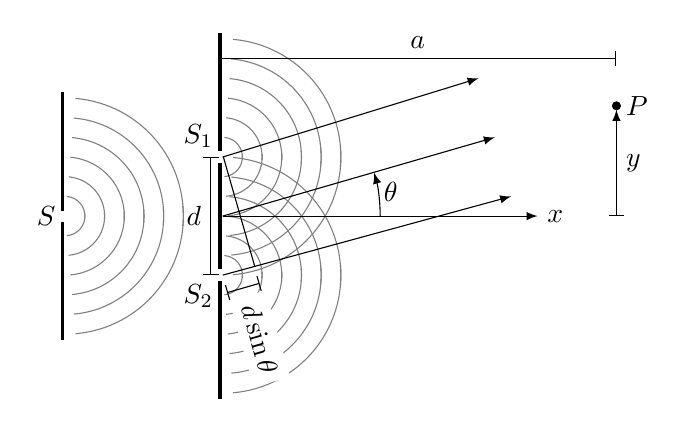
\begin{tikzpicture}[>=latex]
	% first pinhole
	\begin{scope}
		\draw (0,0) node[left] {$S$};
		\foreach \i in {-1,1}
			\draw[xshift=-1,yshift=\i*2,very thick] (0,0) -- (0,\i*1.5);;
		\foreach \r in {1,2,...,6} {
			\draw[scale=\r*.25, rotate=5, color=black!50] (0,-1) .. controls (0.555,-1) and (1,-0.555) .. (1,0);
			\draw[scale=\r*.25, rotate=-5, color=black!50] (0,1) .. controls (0.555,1) and (1,0.555) .. (1,0);
		};
	\end{scope}

	
	% right part
	\begin{scope}[xshift=2cm]
		% pinhole 1
		\begin{scope}[yshift=.75cm]
			\draw (0,0) node[above left] {$S_1$};
			\draw[xshift=-1,yshift=2,very thick] (0,0) -- (0,1.5);
			\draw[xshift=-1,yshift=-2,very thick] (0,0) -- (0,-1.35);
			\foreach \r in {1,2,...,6} {
				\draw[scale=\r*.25, rotate=5, color=black!50] (0,-1) .. controls (0.555,-1) and (1,-0.555) .. (1,0);
				\draw[scale=\r*.25, rotate=-5, color=black!50] (0,1) .. controls (0.555,1) and (1,0.555) .. (1,0);
			};
		\end{scope}

		% pinhole 2
		\begin{scope}[yshift=-.75cm]
			\draw (0,0) node[below left] {$S_2$};
			\draw[xshift=-1,yshift=-2,very thick] (0,0) -- (0,-1.5);
			\foreach \r in {1,2,...,6} {
				\draw[scale=\r*.25, rotate=5, color=black!50] (0,-1) .. controls (0.555,-1) and (1,-0.555) .. (1,0);
				\draw[scale=\r*.25, rotate=-5, color=black!50] (0,1) .. controls (0.555,1) and (1,0.555) .. (1,0);
			};
		\end{scope}
	
		% distance
		\begin{scope}[xshift=-.15cm]
			\draw[|-|] (0,-.75) -- (0,.75) node[pos=.5, left] {$d$};
		\end{scope}
		
		% x-scale
		\draw[thin,->] (0,0) -- (4,0) node[right] {$x$};
		\draw[thin,|-|] (-.05,2) -- (5,2) node[above,pos=.5] {$a$};
		
		% y-scale
		\draw[thin,|->] (5,0) -- (5,1.35) node[right,pos=.5] {$y$};
		\draw[fill=black] (5,1.4) circle (.5mm) node[right]{$P$};
		
		\foreach \i in {0,1,2} {
			\draw[->,yshift=(\i-1)*-.75cm] (0,0) -- (3.25+0.2756*\i*.75,1);
		};
		\draw[rotate=16,xshift=.215cm,yshift=-.725cm] (0,0) -- (0,1.45);
		
		\draw[->] (2,0) arc (0:16:2) node[below right] {$\theta$};
		
		\draw[|-|,rotate=16,yshift=-.95cm] (-0.215,0) -- (0.215,0) node[rotate=-74,pos=.55,right,xshift=.1cm,fill=white] {$d\sin\theta$};
	\end{scope}
\end{tikzpicture}

%				}
		\end{center}
		
		Bei $P$ haben die Strahlen die Phasendifferenz
		\[
			\Delta \Phi = k\cdot d \sin \theta
		\]
		
		Intensitätsmaxima erwartet man, wenn die Phasendifferenz ein ganzzahliges Vielfaches von $2\pi$ beträgt ($\Delta \Phi = \pm 2n\pi$) bzw.~wenn
		\[
			\underbrace{|d \sin \theta|}_{\mathclap{\text{\textbf{Gangunterschied}}}} = n\lambda
		\]
	% subsection das_young_sche_doppelspalt_experiment (end)
	\subsection{Das Prinzip von Huygens} % (fold)
		\emph{Von jedem infinitesimalen Raumelement eines Wellenfeldes geht eine Kugelwelle aus. Die Flächen gleicher Auslenkungen, also die sog.~Wellenflächen, ergeben sich aus der Umhüllenden dieser Kugelwellenflächen.}
		
		\paragraph{Reflexions- und Brechungsgesetz} % (fold)
			\begin{center}
				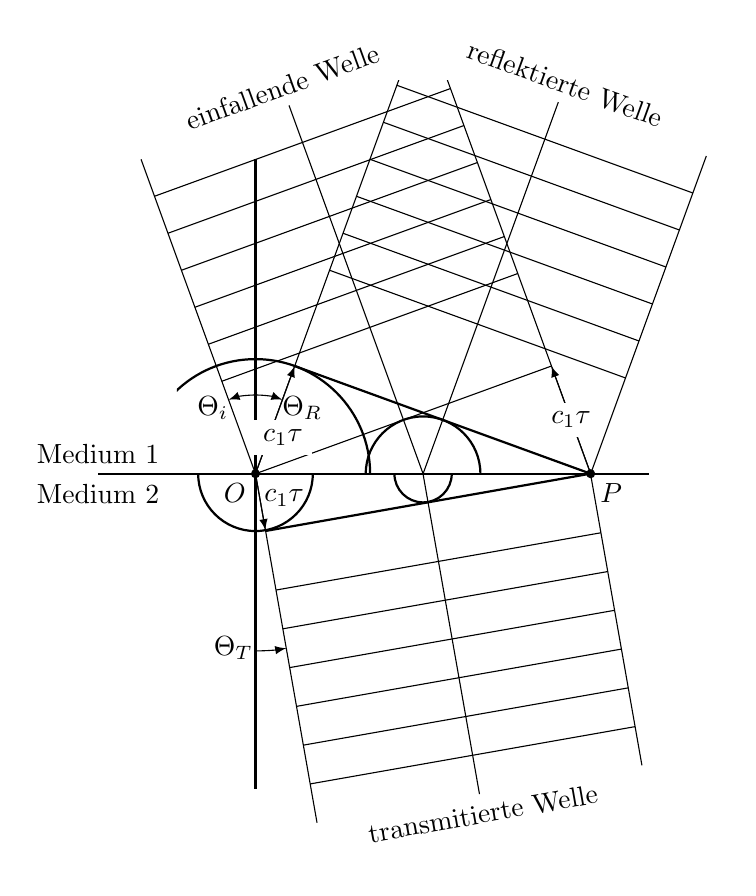
\begin{tikzpicture}[>=latex]
	\begin{scope}
		\clip (-1.5,0) rectangle (6,5);
		\foreach \i in {-1,1} {
			\begin{scope}[rotate=\i*20,yshift=-2cm-\i*.75cm]
				\foreach \i in {0,1,2}
					\draw (\i*2,0) -- (\i*2,7);
				\foreach \i in {0,1,...,5}
					\draw (0,\i*.5+4) -- (4,\i*.5+4);
			\end{scope}
		}
	\end{scope}
	
	\begin{scope}
		\clip (-.01,0) rectangle (5,-5);
		\begin{scope}[rotate=190,yshift=-2.5cm,xshift=-4.19cm,xscale=1.0475]
			\foreach \i in {0,1,2}
				\draw (\i*2,0) -- (\i*2,7);
			\foreach \i in {0,1,...,5}
				\draw (0,\i*.5+4) -- (4,\i*.5+4);
		\end{scope}
	\end{scope}
	
	\begin{scope}
		\draw[thick] (-2,0) node[above]{Medium 1} node[below]{Medium 2} -- (5,0)
		(0,-4) -- (0,4);
		
		\draw[thick,rotate=-20,yshift=1.45588cm] (4,0) -- (0,0);
		\draw[rotate=20,yshift=0cm] (4,0) -- (0,0);
		\draw[thick,rotate=190,yshift=1.45588cm/2+.1mm,xscale=1.0475] (-4,0) -- (0,0);
		
	\end{scope}
	
	\begin{scope}
		\clip (-1,0) rectangle (4,1.5);
		\draw[thick] (0,0) circle (1.45588cm);
		\draw[thick] (2.1284,0) circle (1.45588cm/2);
	\end{scope}

	\begin{scope}
		\clip (-1,0) rectangle (4,-1.5);
		\draw[thick] (0,0) circle (1.45588cm/2);
		\draw[thick] (2.1284,0) circle (1.45588cm/4);
	\end{scope}
	
	\begin{scope}
		\draw[fill=black] (0,0) circle (.5mm) node[below left]{$O$};
		\draw[fill=black] (4.2567,0) circle (.5mm) node[below right]{$P$};
	\end{scope}
	
	\draw[rotate=20,yshift=4.5cm,color=white] (0,0) -- (4,0) node[pos=.5,rotate=20,color=black]{einfallende Welle};
	\draw[rotate=-20,yshift=6cm,color=white] (0,0) -- (4,0) node[pos=.5,rotate=-20,color=black]{reflektierte Welle};
	\draw[rotate=10,yshift=-4.75cm,color=white,xscale=1.0475] (0,0) -- (4,0) node[pos=.5,rotate=10,color=black]{transmitierte Welle};
	
	\draw[->] (0,1) arc (90:110:1cm) node[xshift=-2mm,yshift=-1mm]{$\Theta_i$};
	\draw[->] (0,1) arc (90:70:1cm) node[xshift=2.5mm,yshift=-1mm]{$\Theta_R$};
	\draw[->] (0,-2.25) arc (270:280:2.25cm) node[left,xshift=-3mm]{$\Theta_T$};
	
	\draw[->,rotate=-20] (0,0) -- (0,1.45588cm) node[pos=.3,fill=white,xshift=2mm,yshift=.5mm]{$c_1 \tau$};
	\draw[->,rotate=20,yshift=-1.45588cm] (4,0) -- (4,1.45588cm) node[pos=.5,fill=white]{$c_1 \tau$};
	\draw[->,rotate=10] (0,0) -- (0,-1.45588cm/2) node[pos=.5,xshift=3mm,yshift=.5mm]{$c_1 \tau$};
	
\end{tikzpicture}

			\end{center}
			
			Zur Zeit $t=0$ trifft die Wellenfront bei $O$ ein. Eine Kugelwelle wird erzeugt, die
			sich mit $c_1 = c/n_1$ im Medium 1 und mit $c_2 = c/n_2$ im Medium 2 ausbreitet.
			Zur Zeit $\tau$ trifft die Wellenfront in $P$ ein. Die Kugelwelle im Medium 1 hat den Radius $c_1 \tau$ und im Medium 2 $c_2 \tau$.
			\[
				\Rightarrow \quad \Theta_i = \Theta_R \,,\quad \frac{\sin\Theta_i}{\sin\Theta_T} = \frac{c_1}{c_2} = \frac{n_2}{n_1}
			\]
			
			Kritischer Winkel (vollständige Reflexion):
			\[
				\Theta_c = \arcsin \frac{n_2}{n_1}
			\]
		% paragraph reflexions_und_brechungsgesetz (end)
		\paragraph{Linsen} % (fold)
			\begin{center}
				\vspace{-1cm}
				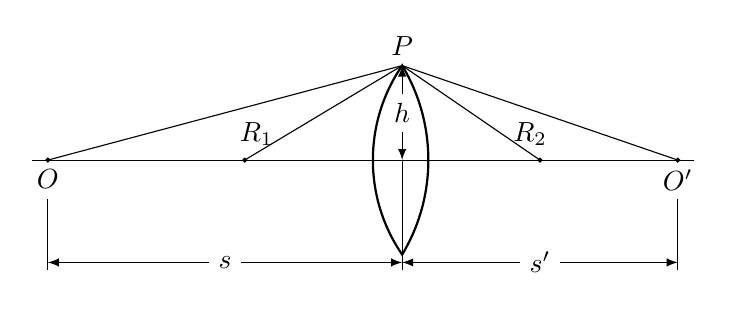
\begin{tikzpicture}[>=latex]
	\draw (3.7,0) -- (-4.7,0);
	\draw[fill=black] (0,1.2) node[above]{$P$} -- (-4.5,0) circle (.25mm) node[below] {$O$};
	\draw[fill=black] (0,1.2) -- (3.5,0) circle (.25mm) node[below] {$O'$};
	\draw (0,-1.4) -- (0,0);
	\draw[<->] (0,1.2) -- (0,0) node[pos=.5,fill=white]{$h$};

	\draw[fill=black] (0,1.2) -- (1.75,0) node[pos=.5,below,xshift=.75cm]{$R_2$} circle (.25mm);
	\begin{scope}
		\clip (0,-1.25) rectangle (-1,1.25);
		\draw[thick] (1.75,0) circle (2.1219cm);
	\end{scope}

	\draw[fill=black] (0,1.2) -- (-2,0) node[pos=.5,below,xshift=-.85cm]{$R_1$} circle (.25mm);
	\begin{scope}
		\clip (0,-1.25) rectangle (1,1.25);
		\draw[thick] (-2,0) circle (2.3324cm);
	\end{scope}
	
	\draw (-4.5,-.5) -- (-4.5,-1.4);
	\draw (3.5,-.5) -- (3.5,-1.4);
	\draw[<->] (-4.5,-1.3) -- (0,-1.3) node[pos=.5,fill=white]{$s$};
	\draw[<->] (3.5,-1.3) -- (0,-1.3) node[pos=.5,fill=white]{$s'$};
\end{tikzpicture}
			\end{center}
			
			\textbf{Linsenmacherformel:}
			\[
				\frac 1 s + \frac 1 {s'} = (n-1) \parens{\frac{1}{R_1} + \frac{1}{R_2}} = \frac 1 f
			\]
			wobei $f$ die Brennweite der Linse ist.
			
			Achsenparallele Strahlen werden in den Brennpunkt fokusiert.
			
			\textbf{Linsenformel:}
			\[
				\frac{y'}{y} = \frac f x = \frac{x'}{f}
			\]
		% paragraph linsen (end)
	% subsection das_prinzip_von_huygens (end)
	\subsection{Die Beugung am Spalt} % (fold)
		Welle durch Spalt mit Dicke $s=\lambda$.
		\begin{align*}
			E_\mathscr{E}(t) &= \frac A s \int_0^s \eu^{\iu(ky \,\sin \phi - \omega t)} \diff y \\
			&= A \,\eu^{\iu(k \frac s 2 \sin \phi - \omega t)} \cdot \frac{\sin(k \frac s 2 \sin \phi)}{k \frac s 2 \sin \phi}
		\end{align*}
		
		Die Intensität variiert mit dem Beobachtungswinkel gemäss
		\[
			I \propto \frac{\sin^2 X}{X^2} \,,\qquad \text{wobei} \quad X = \half k s \sin \phi
		\]
		
		\begin{center}
			%!TEX root = /Users/philipe/Documents/ETH/4. Semester/Physik/Zusammenfassung/Physik II - Zusammenfassung.tex

\begin{tikzpicture}[>=latex,domain=-9.425:9.425,samples=100,xscale=.39,yscale=4]
	\draw[->] (-10,0) -- (10,0) node[right] {$X$};
	\draw[->] (-10,-.15) -- (10,-.15) node[right] {$\sin \phi$};
	\draw[->] (0,-.165) node[below] {$0 \vphantom{\frac \lambda s}$} -- (0,1.1) node[left] {$I$};
	\foreach \i in {-3,-2,-1,1,2,3} {
		\draw (\i*3.1416,.015) -- (\i*3.1416,-.015) node[below] {$\i\pi$};
	};
	\foreach \i in {-3,-2,-1,1,2,3} {
		\draw[yshift=-.15cm] (\i*3.1416,.015) -- (\i*3.1416,-.015) node[below] {$\i\frac{\lambda}{s}$};
	};
	\draw plot[id=intensitaet,smooth] function{sin(x)**2/x**2};
\end{tikzpicture}

		\end{center}
		
		\paragraph{Zusammenhang mit der Fourier-Transformation} % (fold)
			~
			
			Bis auf Konstanten ist die Beugungsamplitude in der Brennebene der Linse (oder unendlich weit weg betrachtet) gleich der Fourier-Transformierten der Durchlässigkeitsfunktion $f(y)$.
			\[
				f(y) = \left\{\begin{array}{rl}
					1 & \text{wenn } |y| \le \frac S 2 \\
					0 & \text{sonst}
				\end{array}\right.
			\]
		% paragraph zusammenhang_mit_der_fourier_transformation (end)
	% subsection die_beugung_am_spalt (end)
	\subsection{Quanteninterferenz} % (fold)
		\paragraph{Einige weitere Grundlagen der Quantenmechanik} % (fold)
			~
		
			In der Quantenmechanik werden \textbf{Observablen} (beobachtbare Grössen) durch \textbf{Operatoren} anstatt Funktionen beschrieben.
		
			\textbf{Energieoperator:}
			\[
				\mathscr H = - \frac{\hbar^2}{2m} \nabla^2 + V(\vec r)
			\]
		
			\textbf{Impulsoperator:}
			\[
				\vec{\tilde{p}} = (\tilde p_x, \tilde p_y, \tilde p_z) = \parens{
					\frac{\hbar}{i} \frac{\partial}{\partial x},
					\frac{\hbar}{i} \frac{\partial}{\partial y},
					\frac{\hbar}{i} \frac{\partial}{\partial z}
				}
			\]
		
			Diese selbst sind nicht messbar, lediglich die Erwartungswerte, welche für einen Operator $A$ definiert sind durch
			\[
				\langle \psi |A| \psi \rangle \equiv \int \psi^* A \,\psi \diff^3 x
			\]
			für den Fall, dass $\psi$ normiert ist (d.h.~$\langle \psi | \psi \rangle = \int |\psi|^2 \diff^3 x = 1$).
		% paragraph einige_weitere_grundlagen_der_quantenmechanik (end)
		\paragraph{Streuung eines quantenmechanischen Teilchens am Spalt} % (fold)
			~
			
			Die Wellenfunktion $\psi(z) = C\cdot \eu^{\iu kz}$ ist ein Eigenzustand des Impulsoperators:
			\[
				\tilde p_z \psi(z) = \hbar k \psi(z) = p_z \psi(z)
			\]
			Der Impuls kann exakt bestimmt werden (Impuls ist \textbf{scharf}). Das Teilchen kann aber nicht exakt lokalisiert werden (sein Ort ist \textbf{unscharf}).
			
			Wellenfunktion als Funktion des Ortes:
			\[
				\psi(y) = \left\{\begin{array}{cl}
					\frac{1}{\sqrt{s}} & \text{für } |y| \le \frac{s}{2} \\
					0 & \text{sonst}
				\end{array}\right.
			\]
			Wahrscheinlichkeit, dass ein Teilchen den Spalt passiert, ist $1$.
			
			Impulsverteilung der Teilchen nach dem sie den Spalt passiert haben (Fourier-Transformation von $\psi(y)$):
			\[
				\phi(p_y) = \frac{1}{\sqrt{2\pi\hbar}} \int_{-\infty}^\infty \psi(y)\, \eu^{-\iu \frac{p_y}{\hbar}y} \diff y
			\]
			
			Wahrscheinlichkeitsdichte, dass ein Teilchen nach dem Spalt mit einem Impuls von $p_y$ erscheint:
			\[
				P(p_y) = |\phi(p_y)|^2
			\]
			
			\subparagraph{Spalt infinitesimaler Breite} % (fold)
				~
				
				Spalt bei $y=y_1$.
				\[
					\phi(p_y) = \frac{1}{\sqrt{2\pi\hbar}} \,\eu^{- \iu \frac{p_y}{\hbar} y_1}
				\]
				\[
					P(p_y) = |\phi(p_y)|^2 = \const
				\]
				Teilchen werden mit gleicher Wahrscheinlichkeit unter jedem Winkel gestreut (vgl.~Kugelwellen nach Spalt).
			% subparagraph spalt_infinitesimaler_breite (end)
			\subsection{Spalt endlicher Breite} % (fold)
				\[
					\phi(p_y) = \frac{1}{\sqrt{2\pi s \hbar}} \int_{-\nicefrac s 2}^{\nicefrac s 2} \eu^{-\iu \frac{p_y}{\hbar}y} \diff y = \sqrt{\frac{2\hbar}{\pi s}} \cdot \frac{\sin\frac{p_y s}{2\hbar}}{p_y}
				\]
				\[
					P(p_y) = |\phi(p_y)|^2 = \frac{2\hbar}{\pi s} \cdot \frac{\sin^2\frac{p_y s}{2\hbar}}{p_y^2}
				\]
			% subsection spalt_endlicher_breite (end)
		% paragraph streuung_eines_quantenmechanischen_teilchens_am_spalt (end)
		\paragraph{Die Unschärferelation von Heisenberg} % (fold)
			besagt, dass
			\[
				\Delta x \Delta p_y = s \frac{2 \pi \hbar}{s} = 2\pi\hbar
			\]
			immer grösser als $\hbar/2$ sein muss.
			
			$\Rightarrow$ Man kann \emph{nie gliechzeitig} Ort und Impuls eines Teilchens exakt bestimmen, lediglich \emph{Wahrscheinlichkeitsaussagen} sind möglich.
		% paragraph die_unschärferelation_von_heisenberg (end)
	% subsection quanteninterferenz (end)
	\subsection{Die Beugung an einem Strichgitter} % (fold)
		$N$ Spalten der Breite $s$ mit Abstand $a$.
		\[
			I \sim \frac{\sin^2(k_y N a/2)}{\sin^2(k_y a / 2)} \cdot \underbrace{\frac{\sin^2(k_y s /2)}{(k_y s / 2)^2}}_{\mathclap{\text{Beugung an einem einzelnen Spalt der Breite $s$}}}
		\]
		Beugungsmaxima treten nur auf bei
		\[
			k_y = n \cdot \frac{2\pi}{a}
		\]
		und werden mit zunehmenden $N$ immer schärfer.
	% subsection die_beugung_an_einem_strichgitter (end)
	\subsection{Compton-Streuung} % (fold)
		Vergrösserung der Wellenlänge eines Photons bei der Streuung an einem Elektron:
		\[
			\Delta \lambda = \frac{h}{mc} (1 - \cos \phi)
		\]
		\begin{tightitemize}
			\item[$\phi$:] Winkel, um den sich die Bewegungsrichtung des Photons durch die Streuung ändert
			\item[$m$:] Masse des Elektrons
		\end{tightitemize}
	% subsection compton_streuung (end)
% section interferenz_und_beugung (end)













































